\documentclass[12pt,compress,aspectratio=169]{beamer}

\usetheme{metropolis}
\setbeamersize{text margin left=.8cm,text margin right=.8cm}

\usefonttheme{professionalfonts}
\usepackage{amsmath,bm}
\usepackage{siunitx}
%\usepackage{graphicx}
\usepackage{tikz}
\usepackage{mathpazo}
\usepackage{xcolor,colortbl}
%\usepackage{hyperref}

\usetikzlibrary{patterns}

\setmonofont{Liberation Mono}
\setlength{\parskip}{0pt}
\setlength{\itemsep}{0pt}
\renewcommand{\baselinestretch}{1}

\sisetup{
  detect-all,
  detect-display-math=true,%  <== NEWLY ADDED
  detect-inline-family=math,% <== NEWLY ADDED
  detect-inline-weight=math,% <== NEWLY ADDED
  number-math-rm=\mathnormal,
  per-mode=symbol
}

\title{Topic 7: Rotational Motion of a Rigid Body}
\subtitle{Advanced Placement Physics C}
\author[TML]{Dr.\ Timothy Leung}
\institute{Olympiads School}
\date{December 7, 2019}

\newcommand{\pic}[2]{\includegraphics[width=#1\textwidth]{#2}}
\newcommand{\mb}[1]{\ensuremath\mathbf{#1}}
\newcommand{\iii}{\bm{\hat{\imath}}}
\newcommand{\jjj}{\bm{\hat{\jmath}}}
\newcommand{\kkk}{\bm{\hat{k}}}
\newcommand{\eq}[2]{\vspace{#1}{\Large\begin{displaymath}#2\end{displaymath}}}


\begin{document}

\begin{frame}
  \maketitle
\end{frame}


%\begin{frame}{Files to Download}
%  Please download the following files from the school website if you have not
%  already done so:
%  \begin{itemize}
%  \item\texttt{PhysAP-06-rotMotion-print.pdf}---The ``print version'' of the
%    class slides for this topic.
%  \item\texttt{PhysAP-06-Homework.pdf}---Homework problems for this topic.
%  \end{itemize}
%  \vspace{.1in}Please download/print the PDF file for the class slides before
%  each class. There is no point copying notes that are already on the slides.
%  Instead, focus on things that aren't necessarily on the slides. If you wish
%  to print the slides, we recommend printing 4 slides per page.
%\end{frame}



\section{Torque}

\begin{frame}{Torque and Rotational Equilibrium}
  Let's consider this question:
  \begin{center}
    \fbox{
      \begin{minipage}{.7\textwidth}
        Two people stand on a board of uniform density. One person has a mass of
        \SI{50}{\kilo\gram} and stands \SI{10}{\metre} away from the fulcrum
        (pivot). The second person has a mass of \SI{65}{\kilo\gram}. How far
        away from the fulcrum would the second person have to stand for the
        system to have to be in equilibrium?
      \end{minipage}
    }
  \end{center}
\end{frame}



\begin{frame}{Equation of Motion}{Newton's Second Law}
  Recall the second law of motion for objects with constant mass:
    
  \eq{-.2in}{
    \mb{F}_\mathrm{net}=m\mb{a}
  }

  \vspace{-.1in}Is it also true for \emph{rotational} motion? If a net force
  $\mb{F}_\mathrm{net}$ causes the center of mass to accelerate (linearly), what
  causes a mass to rotate?

  \vspace{.3in}To answer this, we need to introduce a few concepts first\ldots
\end{frame}



\begin{frame}{Torque}
  I have a rod on a table, and with my fingers, I push the two ends of the rod
  with equal force $\textcolor{red}{F}$. \textbf{What happens?}
  \begin{center}
    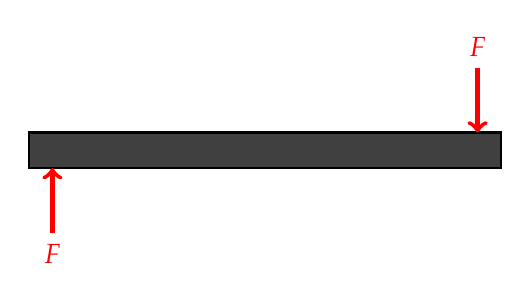
\begin{tikzpicture}[scale=1.5]
      \fill[black!75,draw=black,thick] (-2,-.15) rectangle (2,.15);
      \draw[ultra thick,red,->](-1.8,-.7)--(-1.8,-.15) node[pos=0,below]{$F$};
      \draw[ultra thick,red,->]( 1.8, .7)--( 1.8, .15) node[pos=0,above]{$F$};
    \end{tikzpicture}
  \end{center}
  $\mb{F}_\mathrm{net}=\mb{0}$, therefore $\mb{a}=\mb{0}$. But (obviously) it
  won't stay still either!
\end{frame}



\begin{frame}{What is Torque?}
  \textbf{Torque} (or \textbf{moment}) is the tendency for a force to change
  the rotational motion of a body.
  
  \begin{itemize}
  \item A force $\mb{F}_a$ acting at a point some distance $\mb{r}$ (called the
    \textbf{moment arm}) from a \textbf{fulcrum} (or \textbf{pivot}) at an angle
    $\phi$ between $\mb{F}_a$ and $\mb{r}$
  \item e.g.\ the force to twist a screw
%  \item In the example below, an applied force $\mb{F}_a$ is applied away from
%    the pivot at an angle $\phi$. This generates a torque around the pivot.
  \end{itemize}
  \begin{center}
    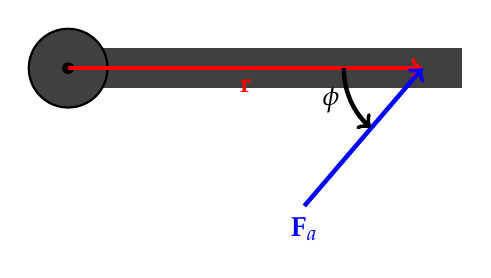
\begin{tikzpicture}[scale=2.5]
      \fill[black!75,draw=black!75] (0,-.1) rectangle (2,.1);
      \fill[black!75,draw=black,thick] (0,0) circle (.2);
      \fill[black] (0,0) circle (.03);
      \draw[ultra thick,red,->](0,0)--(1.8,0) node[midway,below]{$\mb{r}$};
      \draw[ultra thick,blue,->](1.2,-.7)--(1.8,0)node[pos=0,below]{$\mb{F}_a$};
      \draw[ultra thick,->] (1.4,0) arc(180:229:.4)
      node[midway,left]{$\phi$};
    \end{tikzpicture}
  \end{center}
\end{frame}



\begin{frame}{Torque}
  In scalar form, we can express torque $\bm{\tau}$ as the force $\mb{F}_a$,
  the \textbf{moment arm} $\mb{r}$ and the angle $\phi$ between $\mb{F}_a$ and
  $\mb{r}$:

  \eq{-.2in}{
    \boxed{\tau=rF_a\sin\phi}
  }
  
  In vector form, we use the cross-product:

  \eq{-.2in}{
    \boxed{\bm{\tau}=\mb{r}\times\mb{F}_a}
  }
  \begin{center}
    \begin{tabular}{l|c|c}
      \rowcolor{pink}
      \textbf{Quantity} & \textbf{Symbol} & \textbf{SI Unit} \\ \hline
      Torque        & $\bm{\tau}$ & \si{\newton\metre} \\
      Applied force & $\mb{F}_a$  & \si{\newton} \\
      Moment arm (from fulcrum to force) & $\mb{r}$ & \si{\metre}\\
      Angle between force and moment arm & $\phi$ & (no units)
    \end{tabular}
  \end{center}
\end{frame}



\begin{frame}{Torque}
  Going back to the example question:
  \begin{center}
    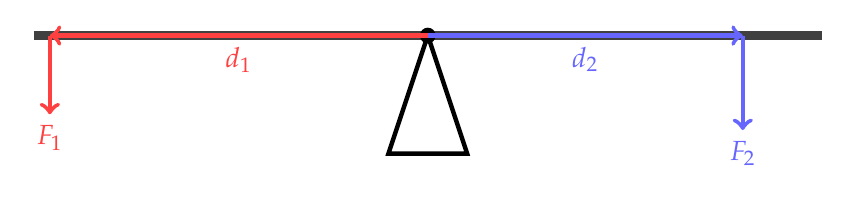
\begin{tikzpicture}
      \fill[black!75,draw=black!75] (-5,-.05) rectangle (5,.05);
      \fill (0,0) circle (.1);
      \draw[ultra thick](0,0)--(.5,-1.5)--(-.5,-1.5)--(0,0);
      \uncover<2->{
        \draw[ultra thick,red!75,->](0,0)--(-4.8,0) node[pos=.5,below]{$d_1$};
        \draw[ultra thick,red!75,->](-4.8,0)--(-4.8,-1)node[pos=1,below]{$F_1$};
      }
      \uncover<3->{
        \draw[ultra thick,blue!60,->](0,0)--(4,0) node[pos=.5,below]{$d_2$};
        \draw[ultra thick,blue!60,->](4,0)--(4,-1.2) node[pos=1,below]{$F_2$};
      }
    \end{tikzpicture}
  \end{center}
  \begin{itemize}
  \item<2->$F_1$ will rotate the board counter clockwise
  \item<3->$F_2$ will rotate the board clockwise
  \item<4->The beam will remain static (in equilibrium) if

    \eq{-.2in}{ F_1d_1=F_2d_2 }
  \end{itemize}
\end{frame}



\begin{frame}{Rotational Equilibrium: First Law of Motion}
  An object is in \textbf{translational equilibrium} is when the force acting
  it is zero, and therefore the acceleration of its center of mass (as
  discussed in Topic 5) is zero:
  
  \eq{-.2in}{
    \mb{F}=\mb{0}
  }

  Having no net force does \emph{not} mean that the object has no translational
  motion; it just means that the object's overall \emph{transtational state} is
  not changing, i.e.\ the translational momentum $\mb{p}$ is constant.
\end{frame}  



\begin{frame}{Rotational Equilibrium: First Law of Motion}
  Likewise, an object is in \textbf{rotational equilibrium} when the net torque
  acting on it is zero:

  \eq{-.3in}{
    \bm{\tau}=\mb{0}
  }
  
  Having no net torque does \emph{not} mean that the object has no rotational
  motion; it just means that the object's overall \emph{rotational state} is
  not changing, i.e.\ $\alpha=\mb{0}$, or that the
  \textbf{angular momentum} $\mb{L}$ is constant.
\end{frame}




\begin{frame}{Example Problem}
  \textbf{Example 8a:} Find the net torque on point C.

  \vspace{-.2in}
  \begin{center}
    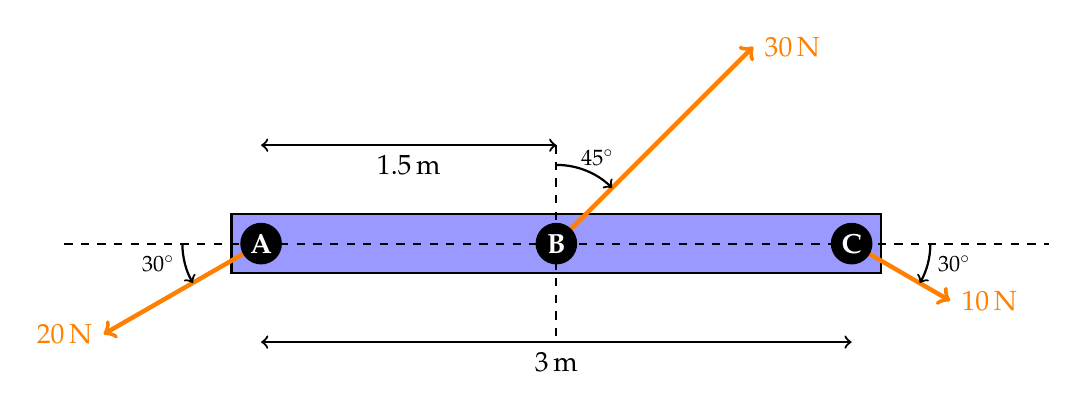
\begin{tikzpicture}[scale=2.5]
      \fill[blue!40!white,draw=black,thick] (-1.65,-.15) rectangle (1.65,.15);
      \draw[thick,<->](-1.5,-.5)--(1.5,-.5) node[midway,below]{\SI{3.}{m}};
      \draw[thick,<->](-1.5,.5)--(0,.5) node[midway,below]{\SI{1.5}{m}};
      \draw[dashed,thick](-2.5,0)--(2.5,0);
      \draw[dashed,thick](0,.5)--(0,-.5);
      \draw[ultra thick,orange,->](0,0)--(1,1)node[pos=1,right]{\SI{30}{N}};
      \draw[thick,->](0,.4)arc(90:45:.4)
      node[pos=.7,above]{\footnotesize\ang{45}};
      \draw[ultra thick,orange,->](-1.5,0)--(-2.3,-.46)
      node[pos=1,left]{\SI{20}{\newton}};
      \draw[thick,->](-1.9,0) arc(180:210:.4)
      node[midway,left]{\footnotesize\ang{30}};
      \draw[ultra thick,orange,->](1.5,0)--(2,-.29)
      node[pos=1,right]{\SI{10}{\newton}};
      \draw[thick,->](1.9,0) arc(0:-30:.4)
      node[midway,right]{\footnotesize\ang{30}};
      \fill[black,draw=black,thick] (-1.5,0) circle(.1);
      \fill[black,draw=black,thick] (   0,0) circle(.1);
      \fill[black,draw=black,thick] ( 1.5,0) circle(.1);
      \node(A) at (-1.5,0) {\color{white}\textbf{A}};
      \node(B) at (0,0) {\color{white}\textbf{B}};
      \node(C) at (1.5,0) {\color{white}\textbf{C}};
    \end{tikzpicture}
  \end{center}
  \uncover<2->{
    \textbf{Example 8b:} Now find the net torque on A.
  }
\end{frame}



\section{Angular Momentum}

\begin{frame}{Angular Momentum}
  Consider a mass $m$ connected to a massless beam rotates with speed $v$ at
  a distance $r$ from the center (shown on the right). It has an
  \textbf{angular momentum} ($\mb{L}$), defined as:
  \begin{columns}
    \column{.77\textwidth}
    
    \eq{-.3in}{
      \boxed{\mb{L}=\mb{r}\times\mb{p}=m(\mb{r}\times\mb{v})}
    }
      
    Or in scalar form:
    
    \eq{-.2in}{
      \boxed{L=rmv}
    }
    \begin{itemize}
    \item $\mb{p}=m\mb{v}$ is the linear/translational momentum
    \item Angular momentum is a vector that depends on the direction of rotation
    \end{itemize}
    
%    \vspace{-.1in}Expanding the terms:
%    
%    \eq{-.4in}{
%      \mb{L}=\mb{r}\times(m\mb{v})=m\mb{r}\times(\bm{\omega}\times\mb{r})
%      =mr^2\bm{\omega}
%    }
%    
%    \vspace{-.2in}Which gives us:
%    
%    \eq{-.3in}{
%      \boxed{\mb{L}=I\bm{\omega}}
%    }
%    
%    \vspace{-.2in}The quantity $I$ is called the \textbf{moment of inertia}.
    
    \column{.23\textwidth}
    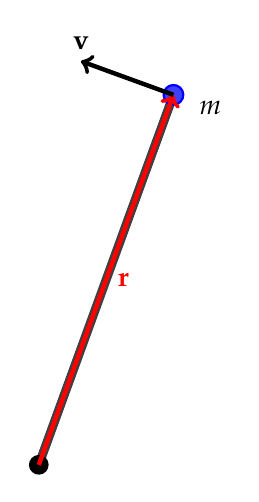
\begin{tikzpicture}[scale=2.5]
      \begin{scope}[rotate=70]
        \fill[black!75,draw=black!75] (0,-.02) rectangle (2,.02);
        \fill[blue!75,draw=blue,thick] (2,0) circle(.05);
        \node(M) at (2,-.2) {$m$};
        \fill[black] (0,0) circle (.05);
        \draw[ultra thick,red,->](0,0)--(2,0)node[pos=.5,right]{$\mb{r}$};
        \draw[ultra thick,->](2,0)--(2,.5)node[pos=1,above]{$\mb{v}$};
      \end{scope}
    \end{tikzpicture}
  \end{columns}
\end{frame}



\begin{frame}{Moment of Inertia}
  A single particle:
  
  \eq{-.2in}{
    \boxed{I=r^2m}
  }

  A collection of particles:

  \eq{-.2in}{
    \boxed{I=\sum r_i^2m_i}
  }

  Continuous distribution of mass:

  \eq{-.2in}{
    \boxed{I=\int r^2dm}
  }
\end{frame}



\begin{frame}{Moment of Inertia}
  \begin{center}
    \pic{.7}{mic.png}
  \end{center}
\end{frame}



\begin{frame}{Angular Momentum and Moment of Inertia}
  \begin{itemize}
  \item Linear and angular momentum have very similar expressions
    
    \eq{-.2in}{
      \mb{p}=m\mb{v}\quad\quad\quad \mb{L}=I\bm{\omega}
    }
  \item Just as $\mb{p}$ describes the overall \emph{translational} state of a
    physical system, $\mb{L}$ describes its overall \emph{rotational} state
  \item Momentum of inertia $I$ can be considered to be an object's
    ``rotational mass''
  \end{itemize}
\end{frame}



\begin{frame}{Second Law of Motion for Rotational Motion}
  \eq{-.35in}{
    \bm{\tau}=\mb{r}\times\mb{F}=\mb{r}\times\frac{d\mb{p}}{dt}
    =\frac{d(\mb{r}\times\mb{p})}{dt}\;\;\longrightarrow\;\;
%      \tau=rF=rm\frac{dv}{dt}=\frac{d(rmv)}{dt}\quad\longrightarrow\quad
%    \end{displaymath}
%    \begin{displaymath}
    \boxed{\bm{\tau} =\frac{d\mb{L}}{dt}}
  }
  \begin{itemize}
  \item If the net torque on a system is zero, then the rate of change
    of angular momentum is zero, and we say that the angular momentum is
    conserved. 
  \item e.g.\ When an ice skater starts to spin and draws his arms inward.
    Since angular momentum is conserved, a decrease in $r$ means an
    increase in $\omega$.
  \end{itemize}
\end{frame}



\begin{frame}{Second Law of Motion for Rotational Motion}
  The second law of motion for rotational motion has a very similar form to
  translational motion:

  \eq{-.2in}{
    \mb{F}=\frac{d\mb{p}}{dt}\quad\quad\bm{\tau}=\frac{d\mb{L}}{dt}
  }

  For objects with constant mass (translational motion) or constant moment of
  inertia (rotational motion), the second law reduces to:

  \eq{-.2in}{
    \mb{F}=m\mb{a}\quad\quad \bm{\tau}=I\bm{\alpha}
  }  
\end{frame}



\begin{frame}{But there is no rotational motion, is there?}
  Even when there is no apparent rotational motion, it does not mean that
  angular momentum is zero! In this case, mass $m$ travels along a straight
  path at constant velocity (uniform motion), but the angular momentum around
  point $P$ is not zero:
  \begin{center}
    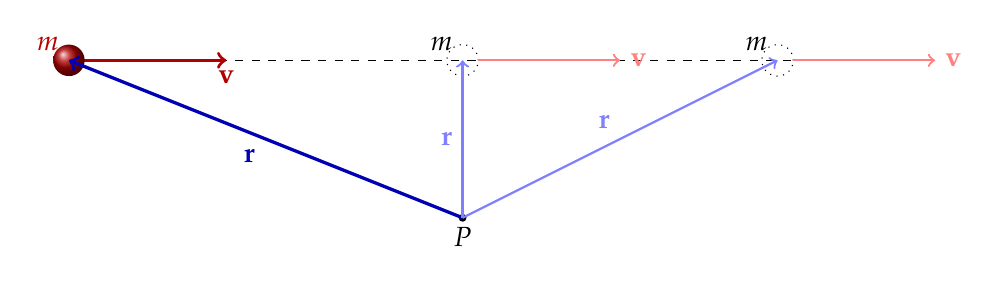
\begin{tikzpicture}
      \draw[dashed](-5,0)--(5,0);
      \draw[very thick,red!70!black,->](-5,0)--(-3,0)
      node[pos=1,below]{$\mb{v}$};
      \tikzstyle{balloon}=[ball color=red!70!black];
      \shade[balloon] (-5,0) circle(.2) node[above left,red!70!black]{$m$};
      \fill[black] (0,-2) circle(.05) node[below]{$P$};
      \draw[very thick,blue!70!black,->](0,-2)--(-5,0)
      node[midway,below left]{$\mb{r}$};
      \uncover<2->{
        \draw[dotted](0,0) circle(.2) node[above left]{$m$};
        \draw[thick,red!50,->](.2,0)--(2,0)node[pos=1,right]{$\mb{v}$};
        \draw[thick,blue!50,->](0,-2)--(0,0) node[midway,left]{$\mb{r}$};
      }
      \uncover<3->{
        \draw[dotted](4,0) circle(.2) node[above left]{$m$};
        \draw[thick,red!50,->](4.2,0)--(6,0)node[pos=1,right]{$\mb{v}$};
        \draw[thick,blue!50,->](0,-2)--(4,0)node[midway,above left]{$\mb{r}$};
      }
    \end{tikzpicture}
  \end{center}
  \uncover<4>{
    Since there is no force and no torque acting on the object, both the linear
    momentum ($\mb{p}=m\mb{v}$) and angular momentum
    ($\mb{L}=\mb{r}\times\mb{v}$) are constant.
  }
\end{frame}



\begin{frame}{Example Problem}
  \textbf{Example 9:} A skater extends her arms (both arms!), holding a
  \SI{2.}{\kilo\gram} mass in each hand. She is rotating about a vertical axis
  at a given rate. She brings her arms inward toward her body in such a way that
  the distance of each mass from the axis changes from \SI{1.}{\metre} to
  \SI{.50}{\metre}. Her rate of rotation (neglecting her own mass) will?
\end{frame}



\begin{frame}{Last Example}
  \textbf{Example 10:} A \SI{1.}{\kilo\gram} mass swings in a vertical circle
  after having been released from a horizontal position with zero initial
  velocity. The mass is attached to a massless rigid rod of length
  \SI{1.5}{\metre}. What is the angular momentum of the mass, when it is in its
  lowest position?
\end{frame}


\begin{frame}{Solving Rotational Problems}
  When solving for rotational problems like the ones described in the previous
  sections:
%  it is imperative to carefully draw a free-body diagram to account
%  for
%all the forces and torques acting on an object, as we have done in the previous
%examples. A few things to keep in mind:
  \begin{itemize}
  \item Draw a free-body diagram to account for all forces
  \item The direction of friction force is not always obvious
  \item The magnitude of any static friction force cannot be assumed to be at
    maximum.
  \item If the object is to change its rotational state, there must be a net
    torque causing it.
  \end{itemize}
\end{frame}



\begin{frame}{Solving Rotational Problems}
  Once the free-body diagram is complete
  \begin{itemize}
  \item Breaks down the \emph{forces} into $\iii$, $\jjj$ and $\kkk$ components
  \item We have now three equations for translation, but it is likely that only
    \emph{one} direction will have forces:

    \eq{-.3in}{
      \sum F_x=ma_x\quad\quad \sum F_y=ma_y\quad\quad \sum F_z=ma_z
    }
  \item And three equations for rotation, and torque is only applied in one
    direction (likely $\kkk$):
    
    \eq{-.3in}{
      \sum\tau_x=I_x\alpha_x\quad\quad \sum\tau_y=I_y\alpha_y\quad\quad 
      \sum\tau_z=I_z\alpha_z
    }
  \end{itemize}
\end{frame}



\begin{frame}{Solving Rotational Problems}
  For rotational motion dynamics equation:
  \begin{itemize}
  \item Relate the force that 
  \item Substitute the expression for momentum of inertia (which has both mass
    and radius terms in it)
  \item Relate angular acceleration to linear acceleration, if applicable:

    \eq{-.35}{
      \alpha=\frac{a}{R}
    }
  \end{itemize}
  Now there are two problems with acceleration terms in
\end{frame}


  
\section{Rotational Kinetic Energy}

\begin{frame}{Rotational Kinetic Energy}
  To find the kinetic energy of a rotating system of particles (discrete number
  of particles, or continuous mass distribution), we sum (or integrate) the
  kinetic energy of the individual particles:
    
  \vspace{-.3in}{\Large
    \begin{align*}
      K&=\sum_i\frac{1}{2}m_iv_i^2=\frac{1}{2}\left(\sum_i m_ir_i^2\right)\omega^2\\
      K&=\int\frac{1}{2}v^2dm=\frac{1}{2}\left(\int r^2dm\right)\omega^2
    \end{align*}
  }
  
  It's no surprise that in both case, rotational kinetic energy is given by:
  
  \eq{-.25in}{
    \boxed{K=\frac{1}{2}I\omega^2}
  }
\end{frame}



\begin{frame}{Kinetic Energy of a Rotating System}
  The total kinetic energy of a rotating system is the sum of its translational
  and rotational kinetic energies at its center of mass:

  \eq{-.2in}{
    \boxed{K=\frac{1}{2}mv_\mathrm{CM}^2+\frac{1}{2}I_\mathrm{CM}\omega^2}
  }
  
  In this case, $I_\mathrm{CM}$ is calculated at the center of
  mass. For simple problems, we only need to compute rotational kinetic energy
  at the pivot:

  \eq{-.2in}{
    \boxed{K=\frac{1}{2}I_\mathrm{P}\omega^2}
  }
  
  In this case, the $I_\mathrm{P}$ is calculated at the pivot.
  \textbf{IMPORTANT:} $I_\mathrm{CM}\neq I_\mathrm{P}$
\end{frame}



\begin{frame}{Parallel Axis Theorem}
  \begin{columns}
    \column{.35\textwidth}
    \pic{1}{Steiner.png}
    
    \column{.65\textwidth}
    The \textbf{parallel axis theorem} relates the moment of inertia of an
    object along two different but parallel axis by:

    \eq{-.2in}{
      \boxed{I=I_{\textrm{CM}}+md^2}
    }
  \end{columns}
\end{frame}
\end{document}
